\begin{CJK}{UTF8}{hei}
\chapter{背景}
\end{CJK}
GTK+和大多数GNOME库因为使用了GObject和比它更低一级的类型系统──GType,从而具有下面的特性:
\begin{itemize}
	\item 面向对象的基于C的API。
	\item 封装成其他编译型语言或动态解释语言的能力。
\end{itemize}
大多数程序员习惯于只使用编译型语言,或者只使用动态解析型语言,却不了解这些语言之间的关联。本文试图向你解释这些疑问,简洁地说明由GLib提供的解决办法。\footnote{即解决编译型语言与解释型语言的沟通问题。}

下面的章节将带你进入一个深层次的理解:关于GType和GObject是如何工作的,作为一个C开发者你将如何使用它们。
\begin{CJK}{UTF8}{hei}
\section{数据类型和编程}
\end{CJK}
关于程序语言的一种说法是:程序语言就是一种创建数据类型并使用函数去操作它们的语言。大多数语言提供了一系例基本类型和一些用于创建更复杂类型的原始类型。

在C语言中,它提供了一些基本类型如char, long, pointer等。在编译C代码的过程中,编译器将这些类型映射至编译器的目标机器的机器类型。如果你正在使用一个C解释器(虽然我从未看到过,不过理论上是有可能的),解释器(用于解释C代码并执行它的程序)在程序运行时,映射这些类型至目标机器的机器类型。

Perl和Python就是那种并不提供类似于C语言的类型的解释型语言。Perl和Python的开发者在操作变量时,变量的类型仅在第一次分配或在第一次使用时被强制为一个类型。解释器也提供一些自动转换的变量类型的方法。例如,在Perl中,一个具有整型值的变量可以在需要时被自动转换成字符串:


\begin{verbatim}
my $tmp = 10;
print "this is an integer converted to a string:" . $tmp . "\n";
\end{verbatim}

当然,在编码中同样允许明确使用一个由语言本身提供的类型转换句式。
\section{导出一个C的API}
C的API是常常是一些从二进制文件中导出的函数集和全局变量。C的函数可以有任意数量的参数和一个返回值。每个函数有唯一的由函数名确定的标识符,并且由C类型来描述参数和返回值。类似的,由API导出的全局变量也是由它们的名字和类型所标识。

一个C的API可能仅仅定义了一些类型集的关联。如果你了解函数调用和C类型至你所在平台的机器类型的映射关系,你可以在内存中解析到每个函数的名字从而找到这些代码所关联的函数的位置,并且构造出一个用在这个函数上的参数列表。最后,你可以用这个参数列表来呼叫这个目标C函数。

为了更好的讨论,请看下面这些C函数的例子和与其相关联在32位x86机器上由gcc产生的汇编代码:
\begin{verbatim}
static void function_foo (int foo)
{}
int main (int argc, char *argv[])
{
    function_foo (10);
    return 0;
}
push $0xa
call 0x80482f4 <function_foo>
\end{verbatim}
函数下显示的汇编代码是非常直观的: 第一个指令在堆栈上建立了十六进制的值0xa(十进制为10)作为一个32位的整型,并调用了function\_foo函数。就如你看到的,C函数的调用由gcc实现成了本地机器码的调用(这是实现起来最快的方法)。

现在,让我来告诉你,一个Python程序是如何调用这个C函数function\_foo的。为了完成调用,Python解释器需要做:

\begin{itemize}
	\item 找到函数所处的位置:这个意味着在C编译器编译成的二进制文件中寻找这个函数。
	\item 在可执行的内存中,载入有关这个函数的相关代码。
	\item 在调用这个函数前,将Python的参数转换为C兼容的参数。
	\item 用正确的方式调用这个函数。
	\item 将C函数的返回值转换成Python兼容的变量并将其返回至Python代码中。
\end{itemize}
上面所描述的处理过程是相当复杂的。不过有几个方法可以使它完全自动化,并且使得其过程对C和Python开发者而言都是透明的:
\begin{itemize}
	\item 第一个解决办法是手动编写一些“粘合代码”,当每个函数被导入或导出时,使用这些代码将Python的参数转换为C兼容的参数,并将C的返回值转换为 Python兼容的返回值。这个粘合代码将被连接到解释器上,从而解释器在解释Python程序时,可以完成程序中的调用C函数的工作。
	\item 另外一个更好的解决办法是自动产生粘合代码,当每个函数被导入或导出时,使用一个特殊的编译器来读取原始的函数签名。
	\item GLib用的解决办法是,使用GType库来保存在当前运行环境中的所有由开发者描述的对象的描述。这些“动态类型”库将被特殊的“通用粘合代码”来自动转换函数参数和进行函数调用在不同的运行环境之间。
\end{itemize}
这个由GType实现的解决方法有很大的优势,在运行环境边界之间的粘合代码只写一次就够了。下图或许会说明的更加清楚:

\begin{figure}[h]
\begin{center}
	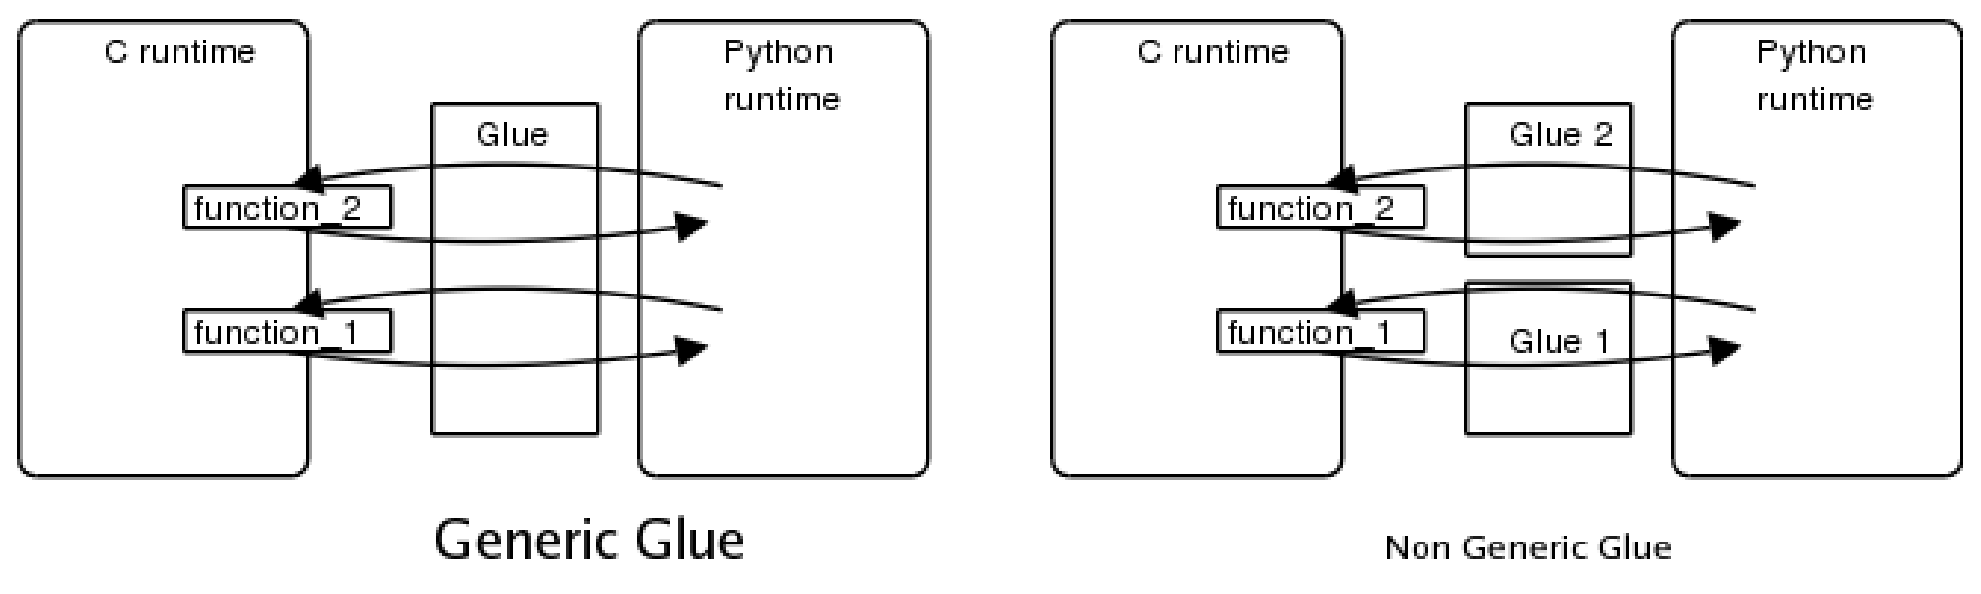
\includegraphics[width=1.0\textwidth]{glue}
	\caption{图}
\end{center}
\end{figure}

当前,至少存在于Python和Perl的通用粘合代码使得直接在Python或Perl使用用GType写的C对象成为可能,只要最少的工作量即可:没有必要去自动或手动去生成巨大的粘合代码。

这个目标被论证是值得称赞的,对它的追求影响了整个GType/GObject库。不过,C开发者很可能会被接下来几章所揭露的特性的复杂性所被难住,如果他们忘了GType/GObject库不仅仅是为了设计向C开发者提供面向对象的特性,也是为了透明的跨语言互通性。
